\documentclass[10pt, compress]{beamer}

\usetheme{m}

\usepackage{booktabs}
\usepackage[scale=2]{ccicons}
\usepackage{minted}

\usepackage{bibentry}
\bibliographystyle{apalike}

\usepgfplotslibrary{dateplot}

\usemintedstyle{trac}

\renewcommand\footnotemark{}
\renewcommand\footnoterule{}

\title{Adding nucleo-olivary inhibition to a bottom-up computational model of the vestibulo-ocular reflex to control gaze stabilization}
\subtitle{}
\date{\today}
\author{Xavier Duran, supervised by Ivan Herreros and Paul Verschure}
\institute{Master in Cognitive Systems and Interactive Media}

\begin{document}

\maketitle

\begin{frame}[fragile]
  \frametitle{Vestibulo-ocular reflex (VOR)}
  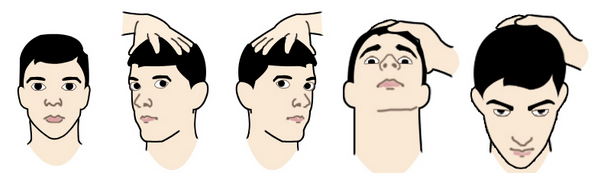
\includegraphics[scale=0.5]{images/vor.png}
  \footnote{\url{http://bit.ly/1Ox3Qd6}}
  This reflex functions to \textbf{stabilize images} on the retinas during \textbf{head movement} by producing \textbf{eye movements} in the direction opposite to head movement, thus preserving the image on the center of the visual field.
\end{frame}

\begin{frame}[fragile]
  \frametitle{VOR adaptation}
  VOR adaptation is controlled by the cerebellum
  \begin{itemize}
    \item CS: head movement
    \item US: retinal slip (error or teaching signal)
    \item CR: corrective eye movements
  \end{itemize}
  \note{Before training in the VOR, image movement across the retina elicits a tracking eye movement response, and head movement elicits the normal VOR eye movement response. During training, head movements (CS) are paired with image movements (US) and these two stimuli together elicit an altered eye movement response which is approximately the sum of the eye movement response to the image movement and the eye movement response to the head movement. Following training, head movement elicits this altered eye movement response in the absence of the visual stimulus (CR). In the second phase of training, the head movement is presented repeatedly in the absence of image movement.}
  \note{paired with a reinforcing unconditioned stimulus }
  \cite{Cohen2004}

  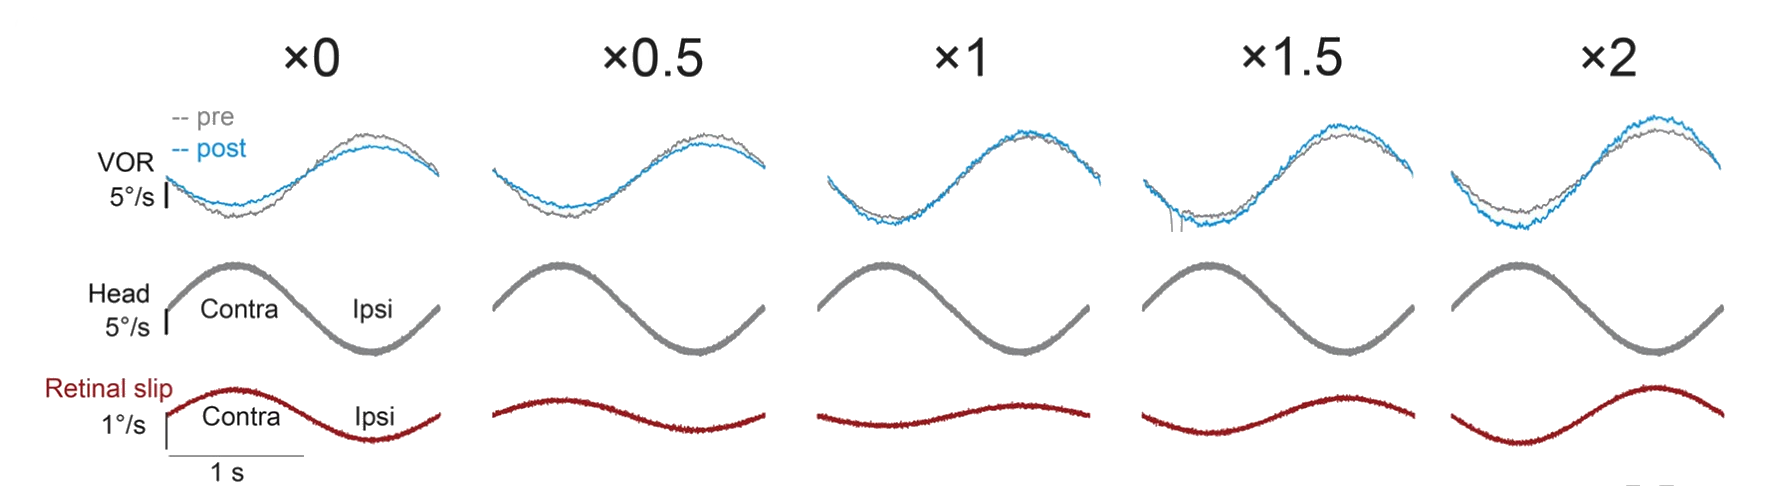
\includegraphics[scale=0.15]{images/guo.png}

  \cite{Guo2014}
\end{frame}

\begin{frame}[fragile]
  \frametitle{Extinction of the learned adaptation}
  \begin{itemize}
    \item old memories may no longer be useful, and in some cases may be maladaptive
    \item learned adaptation is extinguished when no longer necessary
    \item head movements (US) in the absence of visual stimulation (CS) cause a loss of the learned eye movement response (CR)
    \item changes in the amplitude, or gain of the VOR
    \item is mediated by an active, extinction-like process (not by passive forgetting)
  \end{itemize}
  \cite{Cohen2004}

  \note{Classically conditioned eyeblink responses undergo extinction after prolonged exposure to the conditioned stimulus in the absence of the unconditioned stimulus}
  \note{After learning, head movements in the absence of visual stimulation caused a loss of the learned eye movement response. When the learned gain was low, this reversal of learning occurred only when head movements were delivered, and not when the head was held stationary in the absence of visual input, suggesting that this reversal is mediated by an active, extinction-like process}
  \note{It is often adaptive to retain memories over a long period of time. When environmental circumstances change, however, old memories may no longer be useful, and in some cases may be maladaptive. Therefore, an ideal learning system should have a mechanism for suppressing old memories. Old memories can be abolished or suppressed through passive forgetting or through an active process such as extinction, the reduction of a conditioned response that occurs when the learned association between a cue and reinforcement is degraded.}
  \note{we examined whether learned changes in the amplitude, or gain, of the vestibulo-ocular reflex (VOR), a well-studied cerebellum-dependent motor learning paradigm, exhibit a process of reversal analogous to extinction.}
\end{frame}

\begin{frame}[fragile]
  \frametitle{Nucleo-olivary inhibition (NOI): a candidate signal}
  \begin{itemize}
    \item Climbing fibers bring the CS (retinal slip)
    \item Inhibition of climbing fibres serves as a teaching signal for extinction
  \end{itemize}
  \cite{Medina2002}
  \begin{columns}[T]
    \begin{column}[T]{5cm}
      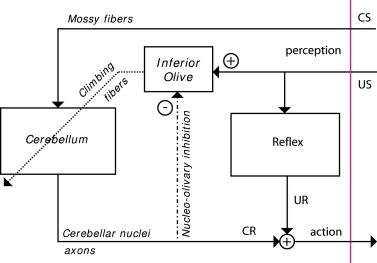
\includegraphics[scale=0.6]{images/noi.jpg}
    \end{column}
    \begin{column}[T]{5cm}
      \begin{itemize}
        \item Cost-optimization
        \item Error-based learning
        \item The gain of the NOI is what determines the amplitude of the response on adaptive reflexes
      \end{itemize}
    \end{column}
  \end{columns}
  \cite{Emken2007, Herreros2013b}
\end{frame}

\begin{frame}[fragile]
  \frametitle{Problem statement}
  \begin{quote}
    State of the art computational models of the vestibulo-ocular reflex don't define a physiological mechanism for extinction
  \end{quote}
\end{frame}

\begin{frame}[fragile]
  \frametitle{Research question}
  \begin{quote}
    Would nucleo-olivary inhibition explain extinction in the vestibulo-ocular reflex computational models?
  \end{quote}
  \begin{block}{Fingerprints}
    \begin{itemize}
      \item NOI has a role in the eye-blink reflex (similar cerebellar circuitry) \cite{Herreros2013b}
      \note{Motor learning in the vestibulo-ocular reflex (VOR) and eyeblink conditioning use similar neural circuitry, and they may use similar cellular plasticity mechanisms.}
      \item There is extinction of the adaptive response in the absence of peripheral error
      \item VOR adaptation has a non-perfect performance, with a residual error proportional to the amount of cerebellar action required
    \end{itemize}
  \end{block}
\end{frame}

\begin{frame}[fragile]
  \frametitle{Hypothesis}
  \begin{quote}
    Adding nucleo-olivary inhibition on a detailed bottom-up state of the art vestibulo-ocular reflex computational model would offer a more
    parsimonious explanation of the experimental behavior of the reflex.
  \end{quote}
\end{frame}

\section{Methods}

\begin{frame}[fragile]
  \frametitle{A bottom-up model computational model of the VOR}
  This computational model is made bottom-up from physiological and behavioral observations
  \begin{itemize}
    \item Plasticity on the cerebellar cortex
    \begin{itemize}
      \item quick
      \item short-term
      \item error-based learning
    \end{itemize}
    \item Plasticity on the brainstem
    \begin{itemize}
      \item slow
      \item long-term
    \end{itemize}
  \end{itemize}
  \cite{Clopath2014}
\end{frame}

\begin{frame}[fragile]
  \frametitle{Learning balance}
  \begin{itemize}
    \item learned adaptation at the cerebellar cortex is slowly transfered to the brainstem
    \item cortical plasticity remains flexible to further adaptations
    \item savings help faster response on reacquisition
  \end{itemize}
\end{frame}

\begin{frame}[fragile]
  \frametitle{Adding NOI to Clopath's model}
  Extinction on Clopath's model
  \begin{itemize}
    \item Weakly modulated by head movement (vestibular signal)
    \item Weights on cortical plasticity experiment a linear decay to their initial value
  \end{itemize}
  Extinction on NOI model
  \begin{itemize}
    \item Extinction is defined as proportional to cortical output \cite{Najac2015}
  \end{itemize}
\end{frame}

\begin{frame}[fragile]
  \frametitle{VOR phase reversal training protocol simulation}
  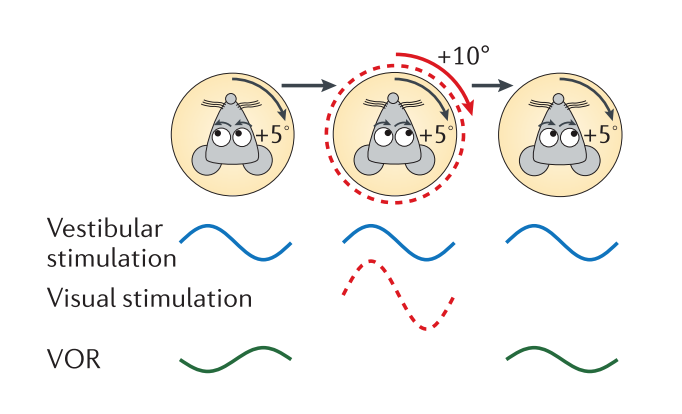
\includegraphics[scale=0.25]{images/vor_adaptation.png}

  \cite{Gao2012a}
  \begin{itemize}
    \item Day 1: VOR cancellation
    \item Day 2: VOR reversal with gain -0.5
    \item Day 3 and 4: Phase reversal with gain -1
    \pause
    \item One week of light deprivation with vestibular stimulation
  \end{itemize}
\end{frame}

\section{Results}

\begin{frame}[fragile]
  \frametitle{Reproducing Clopath's results}
  \begin{columns}[onlytextwidth]
    \column{0.5\textwidth}
      \begin{figure}
        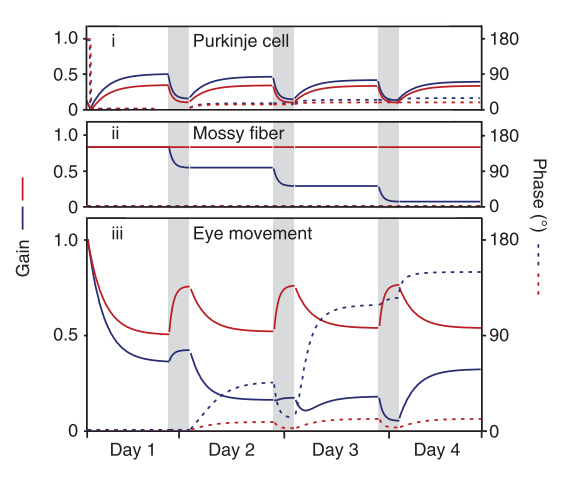
\includegraphics[scale=0.25]{images/gain.png}
        \caption{Experimental results}
      \end{figure}
    \column{0.5\textwidth}
    \begin{figure}
      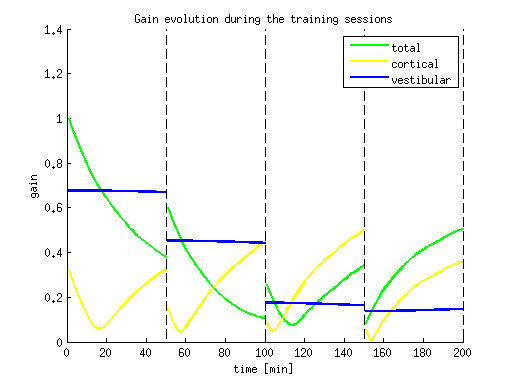
\includegraphics[scale=0.25]{images/longnoi_12.png}
      \newline
      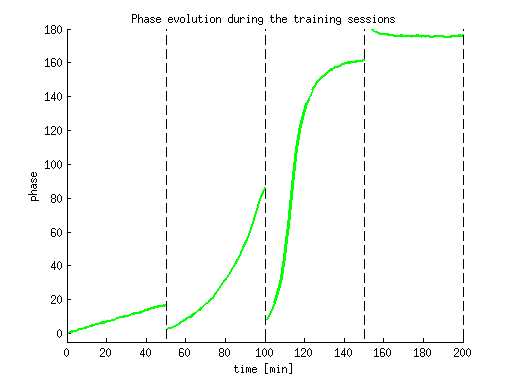
\includegraphics[scale=0.25]{images/longnoi_13.png}
      \caption{Gain and phase on NOI model simulations}
    \end{figure}
  \end{columns}
\end{frame}

\begin{frame}[fragile]
  \frametitle{What happens on the dark?}
  \begin{itemize}
    \item Cortical
      \begin{itemize}
        \item Extinguishes progressively to a baseline
      \end{itemize}
    \item Nuclear
      \begin{itemize}
        \item Continues transference from cortical memory
      \end{itemize}
    \item Total
      \begin{itemize}
        \item Extinction and transference go in different directions
        \item On the dark adaptation continues consolidating until an inflextion point where extinction overtakes transference
        \item After a long period on the dark, all cortical memory is consolidated on the brainstem and cortical contribution is at its baseline
      \end{itemize}
  \end{itemize}
\end{frame}

\begin{frame}[fragile]
  \frametitle{What happens on the dark?}
  \begin{columns}[onlytextwidth]
    \column{0.5\textwidth}
      \begin{figure}
        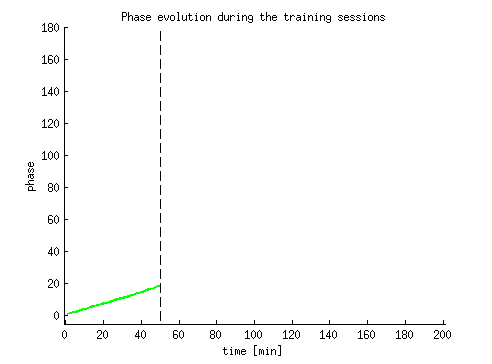
\includegraphics[scale=0.6]{imagesl/longnoi_11.png}
      \end{figure}
    \column{0.5\textwidth}
    Limitations of the model
    \begin{itemize}
      \item control isn't perfect
      \item there's always some modulation on the cortical signal
      \item nuclear transference
    \end{itemize}
  \end{columns}
\end{frame}

\section{Conclusions}

\begin{frame}[fragile]
  \frametitle{Conclusions}
  \begin{itemize}
    \item NOI explains extinction on VOR adaptation
    \item Extinction is triggered when vestibular information is available
    \item Teaching or error signal is modulated by cortical response (OCNO loop)
    \item Savings
  \end{itemize}
\end{frame}

\begin{frame}[fragile]
  \frametitle{Further work}
  More detailed bottom-up models
  \begin{itemize}
    \item transgenic mouse lines
    \item better electro-physiological recordings
    \item models with distributed plasticity
  \end{itemize}
\end{frame}

\section{References}

\begin{frame}[fragile]
  \frametitle{References}
  \bibliography{vornoi}
\end{frame}

\plain{Thank you}

\end{document}
